\section{Network Architecture} \label{sec:netarc}


%=============================================================================%

The LSST Observatory is distributed over four sites: the Summit Site, the Base Site, the Archive Site, 
and the Project Headquarters. While the sites are geographically distributed, they are all functionally 
integrated. Dedicated high-bandwidth fiber optic lines connect the summit and base, with the others 
connected through secure shared networks. Control functions are distributed for operational efficiency 
and to provide robust, reliable, safe operation.

%=============================================================================%

The key driving requirements for the Mountain Summit to the Base Center communications are the 
bandwidth and reliability required to transfer the crosstalk-corrected image data for alert processing and 
the raw image data for forwarding to the Archive Center. Because this link closely follows the path of 
existing CTIO networks, LSST will manage and maintain this mission-critical link, providing the reliability 
and availability necessary to run the combined Mountain-Base infrastructure as a single component of 
the LSST system.

%=============================================================================%

The complete network infrastructure for the LSST has been designed based on existing hardware 
solutions. The network spans several distinct locations as shown in Figure~\ref{fig:global_netarc}. 
The details of the network design are in LSE-78 and details on Information Technology 
and Communication Design can be found in LSE-309. 

%=============================================================================%

\begin{figure}
\begin{center}
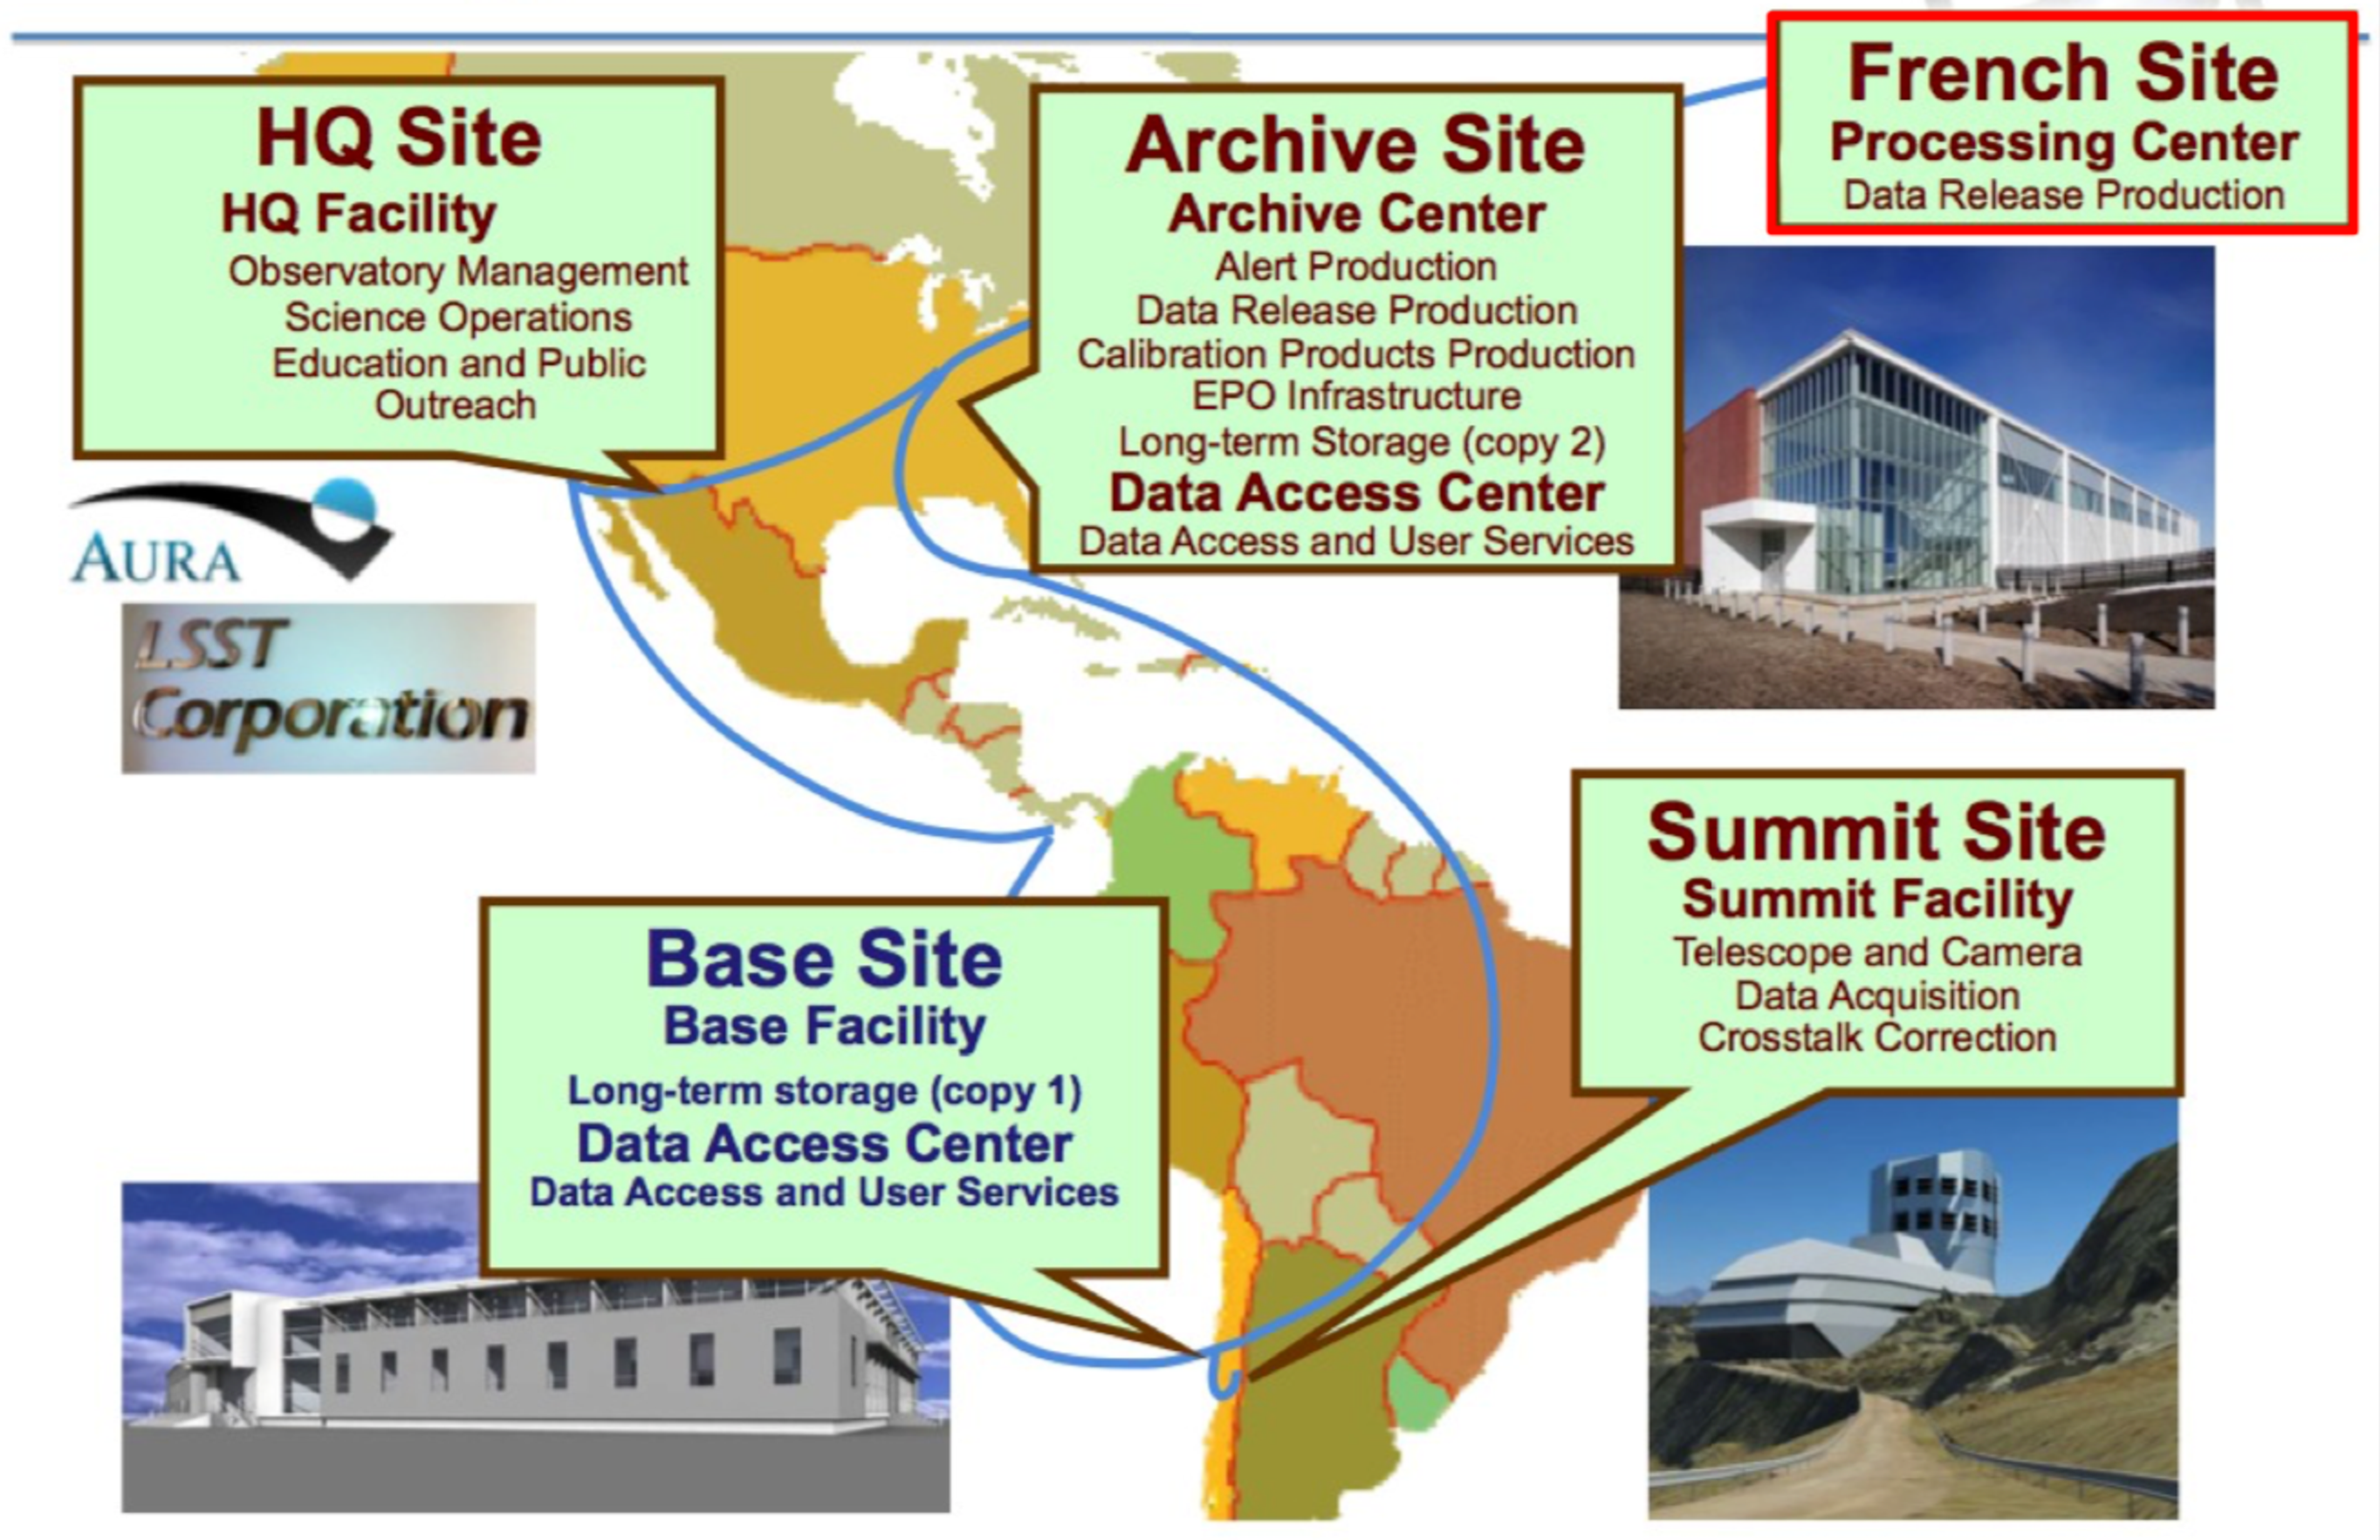
\includegraphics[width=0.6\textwidth]{global_netarc}
\caption{Global network architecture diagram. \label{fig:global_netarc}}
\end{center}
\end{figure}

%=============================================================================%

